\chapter{Analysen}\label{ch:method}

Wie in \cref{ch:usability} bereits erwähnt, liegt eine hohe Usability genau dann vor, wenn ein System von der für es bestimmten Zielgruppe effizient verwendet werden kann.\cite{Richter.2016}
Um dies zu gewährleisten, ist es vorab nötig diese Gruppe zu kennen, zu analysieren und eventuelle Schwierigkeiten in der Benutzung des Systems aufzudecken.
Die Erkennung dieser Schwierigkeiten muss aus Gründen, die ebenfalls in \cref{ch:usability} erläutert wurden, immer in Relation zu der aktuell ausgeführten Aufgabe geschehen.
Aus diesem Grund wird im Folgenden zuerst die Ausgangssituation beschrieben,  in der die Analysen durchgeführt wurden.
Anschließend folgt ein Überblick über die Analysemethoden, bevor abschließend die Ergebnisse dargestellt werden.

\section{Ausgangssituation}
Im ersten Schritt des Human-Centered Design Process, zu sehen in \cref{fig:HCD} des vorherigen Kapitels, gilt es, den Benutzungskontext zu verstehen.
Im Laufe dieses Kapitels wird die Rolle des \textit{User Requirements Engineer} erfüllt, welcher für gewöhnlich für die Dokumentation, Validierung und Verwaltung der Anfoderungen an ein Produkt zuständig ist.
Aus all den möglichen Aufgaben, die in dessen Rolle in diesem Iterationsschritt erfüllt werden sollen, wird in dieser Arbeit auf die Nutzergruppe, deren tägliche Aufgaben und die Arbeitsumgebung genauer eingegangen.

\paragraph{Arbeitsumgebung}
Das Arbeitsumfeld bildet das in \cref{ch:guide} bereits erwähnte EB GUIDE 6.
Es ist hierbei situationsabhängig, ob die Modellierer mit dem Speech-Anteil von EB GUIDE arbeiten oder nicht.
Für diese Arbeit werden die Interaktionen mit dem Speech-Anteil ignoriert und sich nur auf die Usability von EB GUIDE Studio konzentriert.
Auch auf beide Target Frameworks wird im Folgenden nicht mehr weiter eingegangen, da die Nutzerinteraktion mit EB GUIDE über die Schnittstelle EB GUIDE Studio stattfindet.

\paragraph{Nutzergruppe}
Die Zielgruppe für die Analysen im Rahmen dieser Arbeit deckt sich  mit der Nutzergruppe von EB GUIDE.
Im Rahmen dieser Arbeit wurden nur Personen beobachtet und analysiert, die bei Elektrobit beschäftigt sind.
Aus den getätigten Beobachtungen geht hervor, dass die Nutzer teilweise sehr routiniert und auch täglich mit der Software arbeiten, andere benötigen diese hingegen nur sporadisch in ihrer Arbeit.
Es werden also Experten und gelegentliche Nutzer in dieser Arbeit untersucht, Nutzer die noch nie mit der Software gearbeitet haben, werden nicht beachtet.
Wie in \cref{ch:usability} dargestellt, ergibt sich hieraus die Möglichkeit, das System auf Effizienz, Wiedererkennungswert, Fehler und Zufriedenheit zu testen, welche jedoch im Folgenden noch eingegrenzt werden.

\paragraph{Arbeitsaufgaben}
Der Großteil der Modellierer arbeitet in laufenden Projekten von Elektrobit und modelliert dort mithilfe von EB GUIDE 6 Human Machine Interfaces für die Automobilbranche.
Ein anderer Teil der Zielgruppe arbeitet an Kundendemonstrationen, mit deren Hilfe dargestellt wird, was mit der aktuellen Version von EB GUIDE 6 modelliert werden kann.
Beide Gruppen setzen bei ihrer Arbeit Spezifikationen um, die nach den Wünschen des Kunden direkt von diesem oder von Designfirmen erstellt werden.
Diese Spezifikationen bestehen meist aus einem schriftlichen Teil, der die Logik beschreibt, nach der das Interface arbeiten muss, sowie aus einem grafischen Teil, der die Anordnung von Icons und Texten darstellt.

\section{Vorgehensweise}
Nachdem nun der Benutzungskontext analysiert wurde, gilt es im zweiten Schritt des Prozesses, die Benutzeranforderungen zu spezifizieren.
Diese Benutzeranforderungen sind testbar, eindeutig, konsistent und beinhalten die Definition identifizierter Bedürfnisse der Nutzer.
Zu unterscheiden sind qualitative und quantitative Benutzeranforderungen, wobei beide eine Basis für das Design des interaktiven Systems bieten und durch Evaluierung des Systems verifiziert werden können.
Qualitative Anforderungen beziehen sich auf die Art und Weise wie das System genutzt wird, um das Ziel zu erreichen, quantitative Anforderungen hingegen setzen messbare Ziele für die Usability und User Experience.\cite{.f}

Um repräsentative Benutzeranforderungen zu erhalten, ist es notwendig, dass die Bedürfnisse der Nutzer, aus denen die Anforderungen gebildet werden, tatsächlich auch den Bedürfnissen der Zielgruppe entsprechen.
Diese Bedürfnisse erhält man beispielsweise durch Interviews oder Beobachtungen innerhalb der Zielgruppe.
Diese Vorgehensweisen werden im Rahmen dieser Arbeit kombiniert angewandt, wodurch die Rollen \textit{Interviewer} und \textit{Beobachter} auf eine Person reduziert werden.
Die Nutzer werden bei ihrer täglichen Arbeit beobachtet und währenddessen aufgefordert, ihre aktuellen Arbeitsschritte zu erklären, wodurch sie bei Bedarf auch automatisch Kritik am Interface äußern können und dem Beobachter/Interviewer begleitendes Befragen ermöglicht wird.

\section{Ergebnisse}
\label{ch:results}
Die soeben beschriebenen Vorgehensweise wird bei der Beobachtung/Befragung von fünf Modellierern angewandt.
Da hier immer der gesamte Ablauf einer typischen Arbeitsaufgabe beobachtet wird, variiriert die Dauer der Sitzungen.
Im Durchschnitt werden die Modellierer jedoch 2 bis 3 Stunden bei ihrer täglichen Arbeit beobachtet und währenddessen zu - für den Beobachter unklaren - Abläufen befragt.
Bei der Durchführung der Beobachtungen fallen einige Dinge auf, die die Modellierer bei ihrer Arbeit behindern oder erheblich verlangsamen und welche alle in den folgenden Abschnitten aufgeführt werden.
Teilweise fällt den Nutzern das selbst auf und sie weisen den Beobachter darauf hin; teilweise haben sie sich bereits so an die Arbeitsschritte gewöhnt, dass die Behinderung nur einem Außenstehenden auffällt, den Nutzern selbst jedoch nicht mehr.

Im Folgenden werden zuerst Beobachtungen allgemein erläutert, bevor die Bedürfnisse der Nutzer formuliert werden, damit es abschließend möglich ist, die qualitativen Benutzeranforderungen zu definieren.
Die Quantitativen Anforderungen werden in \cref{ch:outlook}, im Rahmen des tatsächlichen Usability Tests, aufgeführt.

\paragraph{Image List}
Bei einer Image List handelt es sich um ein Datapool Item. 
Datapool Items sind Modelelemente, die benutzt werden können, um Daten von der Applikation an das Interface zu senden, oder umgekehrt.
Außerdem können damit Daten gespeichert werden, die entweder nur von Seiten des Interfaces genutzt werden, oder nur von der Applikationsseite\cite{studio_guide}.
In \cref{tab:gt} kann das Befüllen eines solchen Datapool Items am Beispiel einer Image List nachvollzogen werden.

\newpage

\begin{longtable}[H] { c | m{5cm} }
\hline
Arbeitsschritt & Beschreibung \\ \hline 
\\
  \centering
 % \begin{tabular}{ c | m{5cm} }
    \begin{minipage}{.25\textwidth}
      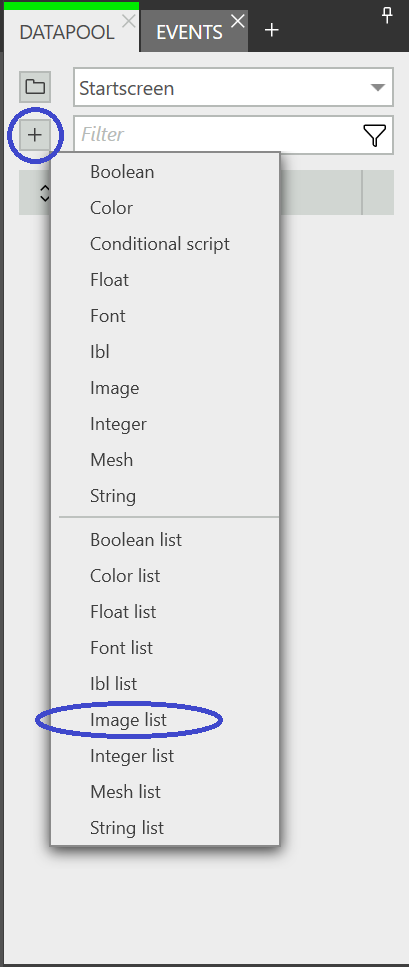
\includegraphics[width=\linewidth]{figures/ImageList_01.PNG}
    \end{minipage}
    &
    %\begin{minipage}[t]{5cm}
   Anfangs besteht für den Nutzer die Möglichkeit, aus einer Vielzahl von Datapool Items zu wählen.
  Hierfür werden bereits zwei Klicks benötigt, dieser Vorgang ist jedoch einmalig und kann auch nicht reduziert werden
    %\end{minipage}
    \\ 
    \\ \hline
    \\
 \begin{minipage}{.25\textwidth}
      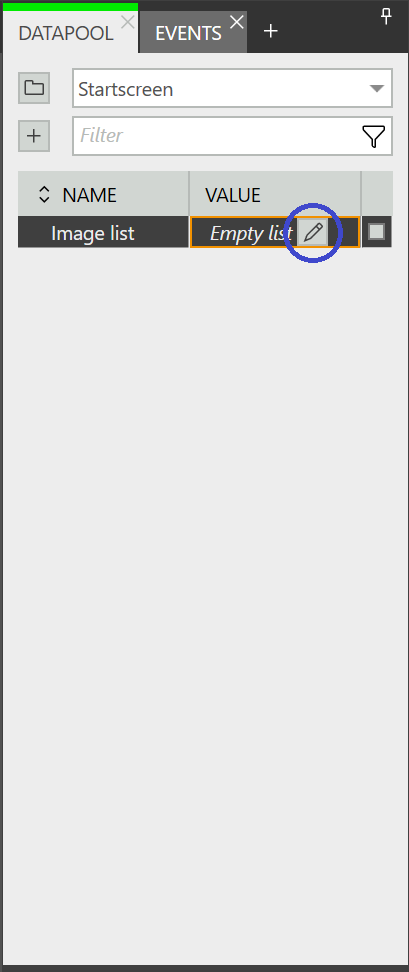
\includegraphics[width=\linewidth]{figures/ImageList_02.PNG}
    \end{minipage}
    &
    %\begin{minipage}[t]{5cm}
   Hier initialisiert der Nutzer das Befüllen der Liste durch einen Klick auf den \glqq Stift\grqq{} Button, wodurch sich das Pop Up in der Folgenden Grafik öffnet.
    %\end{minipage}
	\\	
 \\ \hline
    \\
 \begin{minipage}{.4\textwidth}
      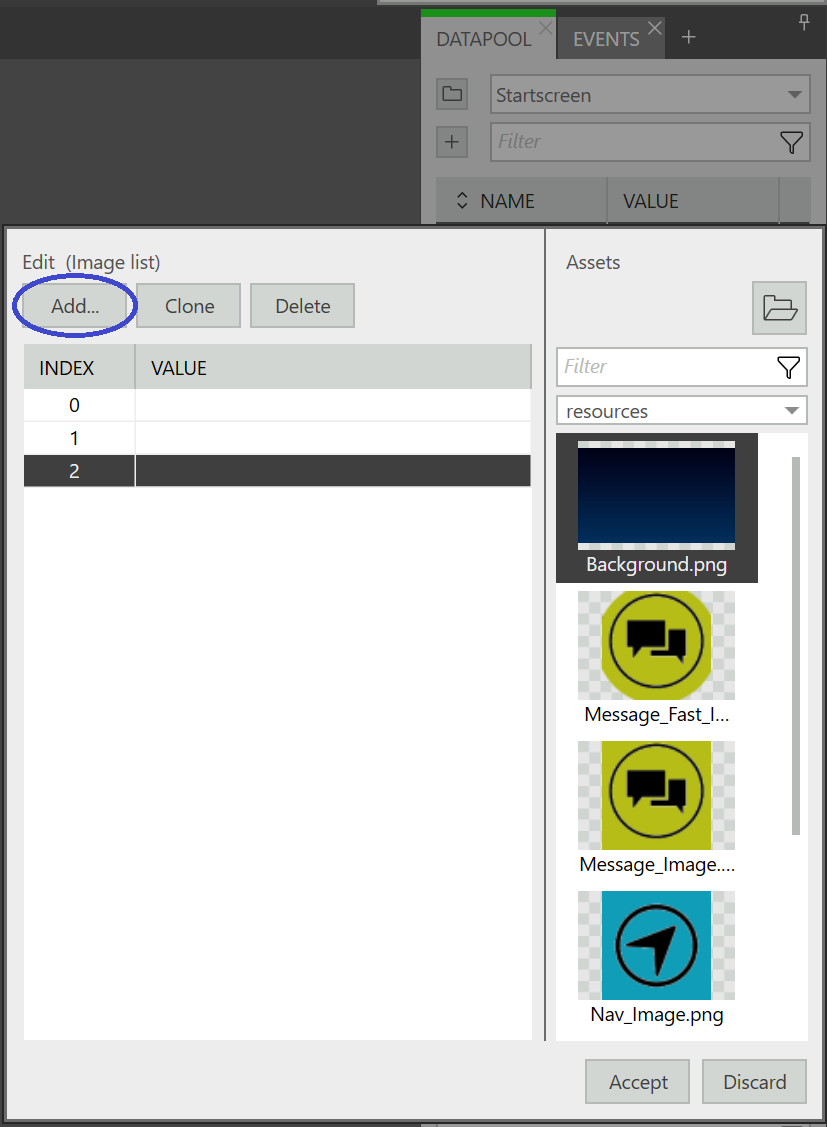
\includegraphics[width=\linewidth]{figures/ImageList_04.PNG}
    \end{minipage}
    &
    %\begin{minipage}[t]{5cm}
   Die hier zu sehenden Platzhalter für Index und Value müssen einzeln durch einen Klick auf den \glqq Add..\grqq{} Button hinzugefügt, ...
    %\end{minipage}
	\\	
 % \end{tabular}
 \\ \hline
    \\
 \begin{minipage}{.4\textwidth}
      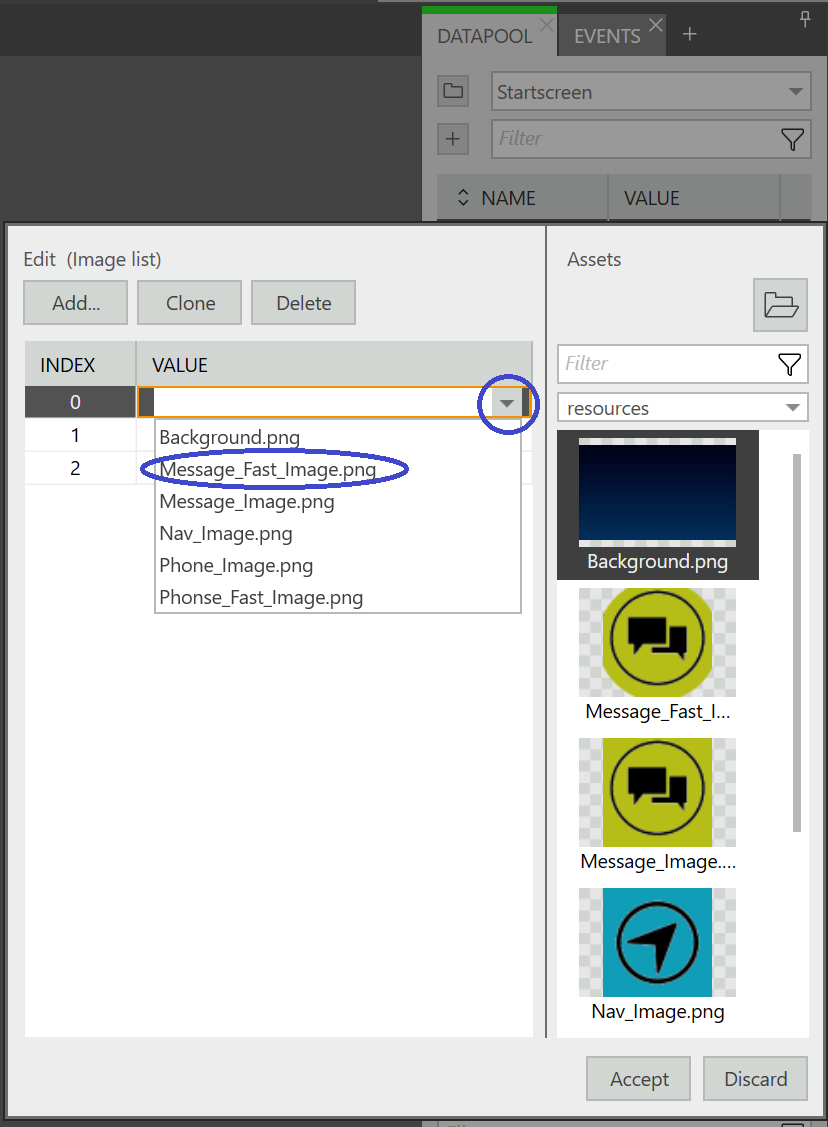
\includegraphics[width=\linewidth]{figures/ImageList_05.PNG}
    \end{minipage}
    &
    %\begin{minipage}[t]{5cm}
  ... und danach individuell mit dem gewünschten Images befüllt werden.
    %\end{minipage}
	\\	
 % \end{tabular}
\\
  \caption{Usability - Schwäche Image List}\label{tab:gt}
\end{longtable}

%In Abbildung b) initialisiert der Nutzer das Befüllen der Liste durch einen Klick auf den \glqq Stift\grqq{} Button, wodurch sich das Pop Up in Abbildung c) öffnet.
%Die hier zu sehenden Platzhalter für Index und Value müssen einzeln durch einen Klick auf den \glqq Add..\grqq{} Button hinzugefügt werden, und danach, wie in Abbildung d) markiert, mit dem gewünschten Image befüllt werden.
Für die minimale Auswahl in diesem Beispiel ist der Aufwand noch überschaubar, es gilt jedoch zu bedenken, dass in tatsächlichen Projekten Image Lists mit mindestens 100 Images erstellt werden.
Das bedeutet für den Nutzer mehrere Stunden Arbeit, die keinen wirklichen Mehrwert liefern und den Joy of Use deutlich mindern.
Joy of Use bezeichnet im Allgemeinen eine Erweiterung der Usability und beschreibt die positiven Erfahrungen eines Nutzers.
Diese werden vor allem durch das effiziente Erreichen der gesteckten Ziele erreicht, was bei einer sich immer wieder wiederholenden Tätigkeit nicht gegeben ist.

%\begin{figure}

%  \centering
%  \subfloat[][]{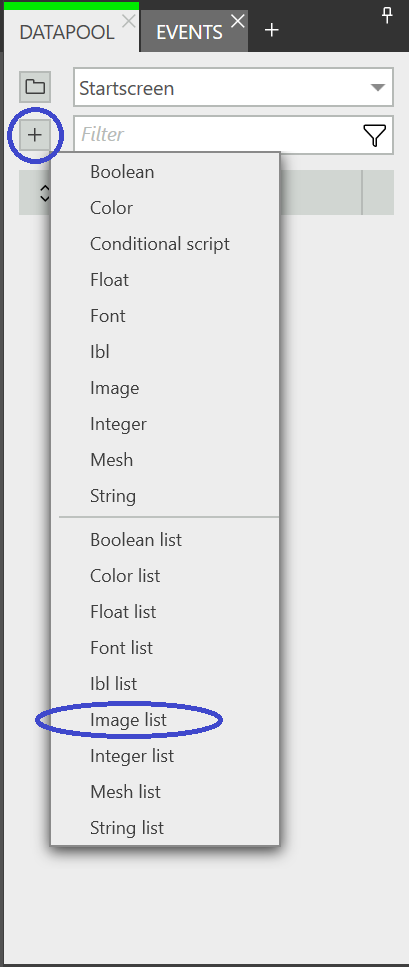
\includegraphics[width=0.3\linewidth]{figures/ImageList_01.PNG}}%
%  \qquad
%  \subfloat[][]{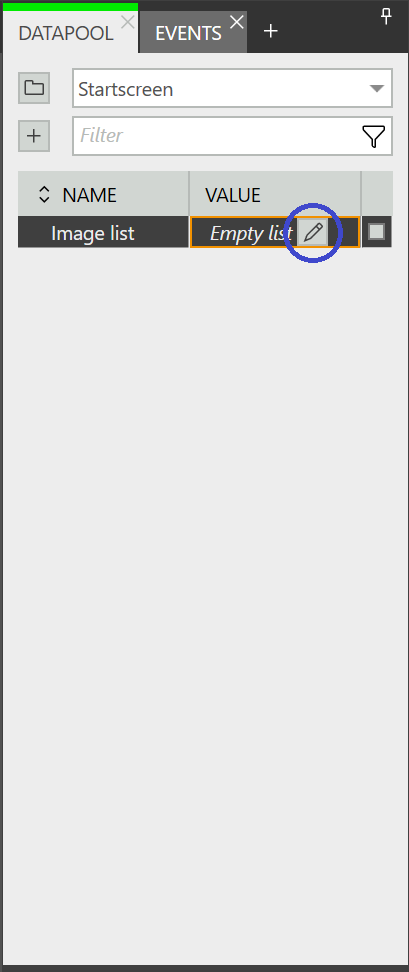
\includegraphics[width=0.3\linewidth]{figures/ImageList_02.PNG}}%
% \qquad
%  \subfloat[][]{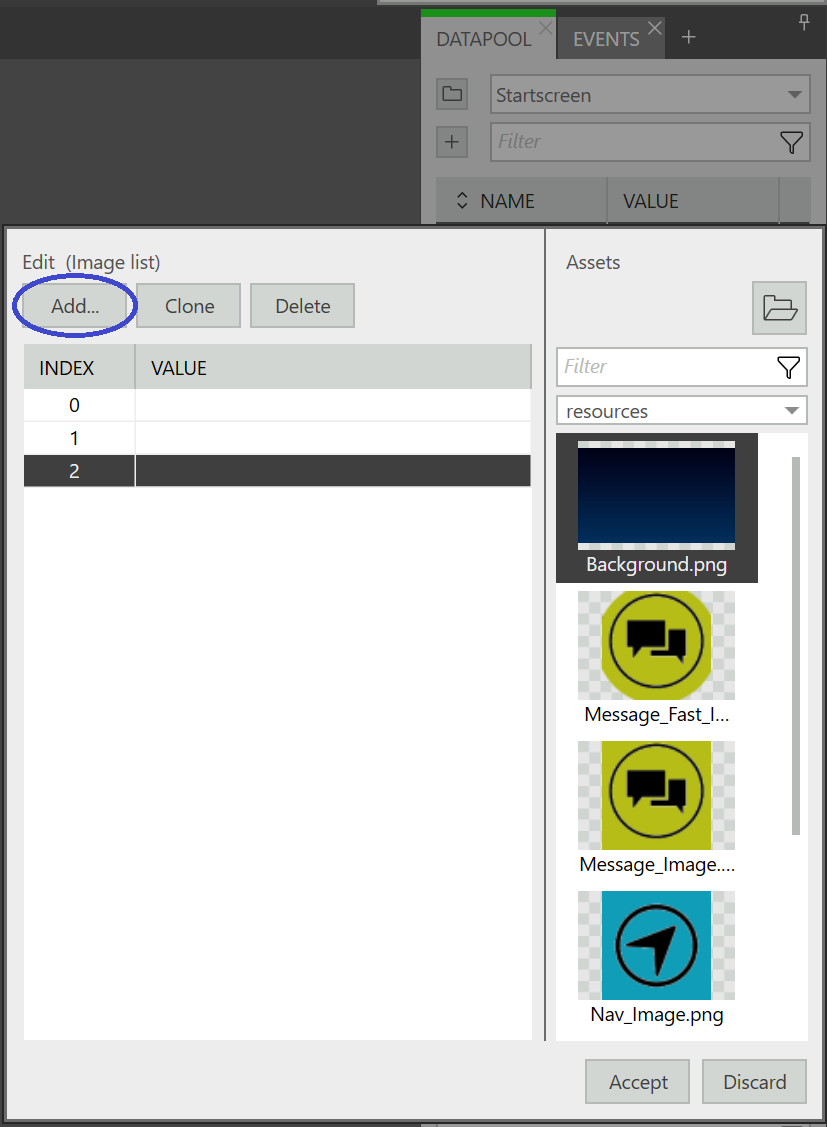
\includegraphics[width=0.4\linewidth]{figures/ImageList_04.PNG}}%
% \qquad
%  \subfloat[][]{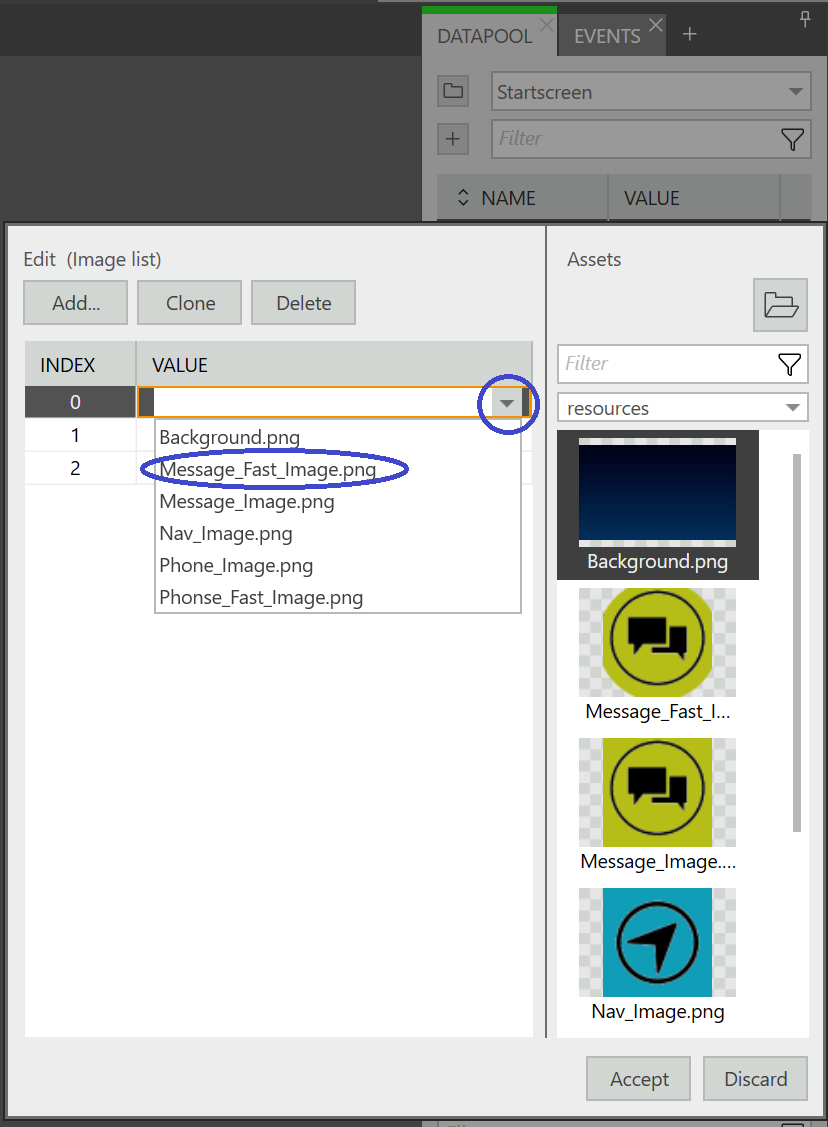
\includegraphics[width=0.4\linewidth]{figures/ImageList_05.PNG}}%
%  \caption{Usability - Schwäche Image List}%
%  \label{fig:ImageList}
%\end{figure}

\paragraph{Resultierende Benutzeranforderung}
Nutzer, die eine Datapool Liste anlegen, müssen die Möglichkeit haben, mehrere Images gleichzeitig zu dieser Liste hinzuzufügen.

\paragraph{Navigation}
Soll ein neues Element in der View hinzugefügt werden, wird der Widget Tree in der Navigation, in \cref{fig:Navigation} zu sehen, nicht automatisch ausgeklappt.
Durch Beobachtung kann festgestellt werden, dass die Nutzer, nachdem sie ein neues Element eingefügt haben, dieses sofort umbenennen. 
Für diesen Vorgang muss das Element im Widget Tree erst gesucht werden, wobei sich, je nach angelegten Ebenen im Projekt, die Anzahl der hier benötigten Klicks exponentiell steigert.
Sollte der Nutzer in \cref{fig:Navigation} beispielsweise gerade das NavImage eingefügt haben, müssen erst vier Ebenen ausgeklappt werden, bevor das Umbenennen möglich ist.
In größeren Projekten ist es üblich, mehrere Templates ineinander zu schachteln, was bis zu 10 Ebenen im Widget Tree führen kann.
Ein automatisches Ausklappen desselbigen, würde den Nutzern also vor allem in komplizierteren Projekten unnötigen Aufwand ersparen.

\begin{figure}[H]
  \centering
  \subfloat[][]{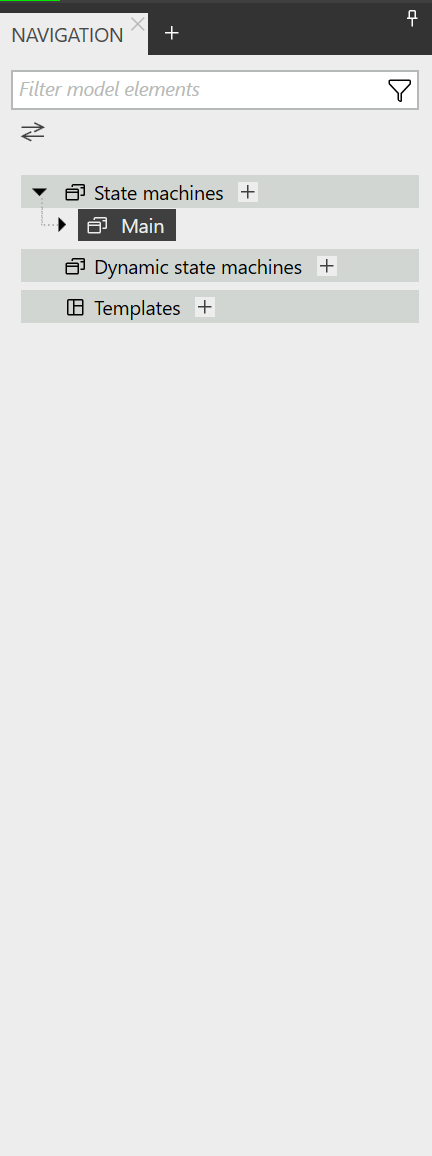
\includegraphics[width=0.25\linewidth]{figures/Navigation.png}}%
  \qquad
  \subfloat[][]{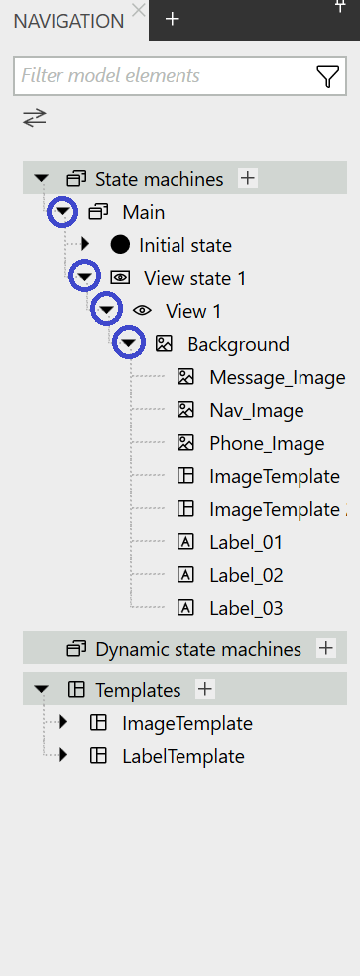
\includegraphics[width=0.25\linewidth]{figures/Navigation_01.png}}%
  \caption{Usability - Schwäche Navigation}%
  \label{fig:Navigation}
\end{figure}

\paragraph{Resultierende Benutzeranforderung}
Nutzer, die ein neues Element zu ihrer View hinzufügen, müssen die Position dieses Items sofort im Widget Tree nachvollziehen können.

\paragraph{Template Properties}
Ein Widget Template ermöglicht die Definition eines individuellen Widgets, welches beliebig oft in einem EB GUIDE Model benutzt werden kann.
Es besteht die Möglichkeit, Templates zu erstellen, die auf bereits existierenden Widgets aufbauen oder von einem anderen Template abgeleitet sind.
Nach der Erstellung kann das Template nach den eigenen Wünschen und Bedürfnissen angepasst werden, beispielsweise durch das Hinzufügen von Properties.

Ein Widget Template besitzt außerdem ein Template Interface, welches jene Properties des Templates beinhaltet, die für jede Instanz des Templates sichtbar und veränderbar sein sollen.
Jede Instanz eines Templates erbt also die Properties des Template Interfaces.
Diese werden Template Properties genannt.\cite{studio_guide}

In \cref{fig:TemplateProperties} ist zu sehen, wie die Funktion \glqq publish to template interface\grqq{} ausgeführt wird.
Hierfür ist zuerst ein Rechtsklick auf das Viereck hinter dem gewünschten Property nötig, bevor noch auf \glqq Add to template interface\grqq{} geklickt werden muss.
Während der Beobachtung wird deutlich, dass vor allem der Rechtsklick den Arbeitsablauf sehr beeinträchtigt, da dieser in EB GUIDE selten verwendet wird. 
Zum Großteil wird mit dem normalen Linksklick gearbeitet, weshalb das auch für diesen Fall wünschenswert wäre.
In Teil b) von \cref{fig:TemplateProperties} sieht man, dass das verlinkte Property nun einen blauen, statt einem weißen Kreis aufweist.
Alle anderen Optionen, wie  \glqq Add link to widget property\grqq{} wirken sich nach ihrer Anwendung farblich auf das eben angeklickte Quadrat und nicht auf den Kreis aus.
Es wäre also denkbar, die Funktion \glqq publish to template interface\grqq{} einfach durch einen Linksklick auf den Kreis zu aktivieren.

\begin{figure}[H]
  \centering
  \subfloat[][]{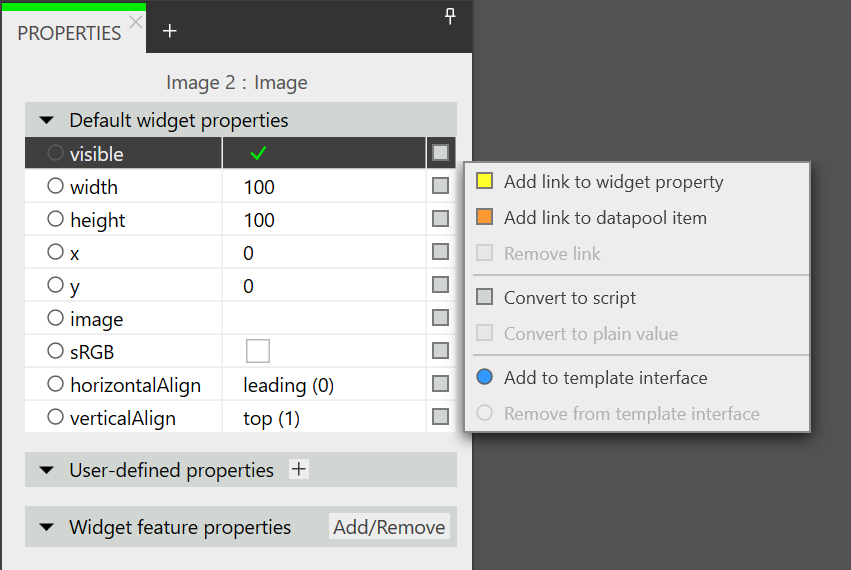
\includegraphics[width=0.5\linewidth]{figures/TemplateProperties.png}}%
  \qquad
  \subfloat[][]{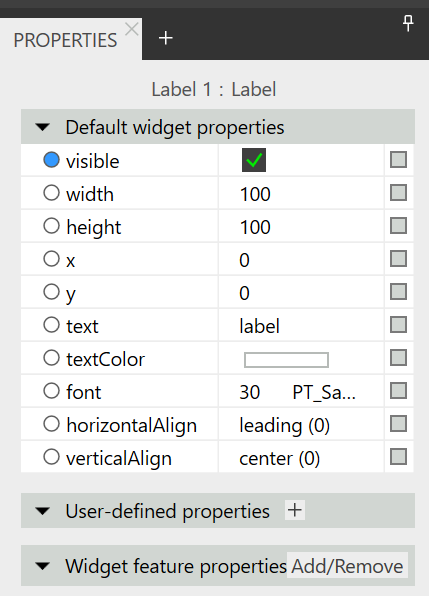
\includegraphics[width=0.3\linewidth]{figures/TemplateProperties_01.png}}%
  \caption{Usability - Schwäche Template Properties}%
  \label{fig:TemplateProperties}
\end{figure}


\paragraph{Resultierende Benutzeranforderung}
Nutzer, die für ein Property die Funktion \glqq publish to template interface\grqq{} ausführen möchten, müssen dies auf eine intuitive und direkte Art und Weise tun können.

\paragraph{Widget Feature Properties}

Neben den Default Widget Properties wie Breite und Höhe, die jede Widgetinstanz besitzt, existieren noch die so genannten Widget Feature Properties.
Diese Features fügen weitere anpassbare Funktionen für das Aussehen und Verhalten der Widgets hinzu.
Wie in \cref{fig:WidgetFeatureProperty} zu sehen, sind die Features in Kategorien unterteilt, die grafisch in Form eines Dropdownmenüs dargestellt sind.

Bei der Beobachtung der Nutzer fällt auf, dass viele genau wissen, welches Feature sie hinzufügen wollen, jedoch häufig die zugehörige Kategorie nicht präsent haben.
Dies führt dazu, dass jedes Dropdownmenü aufgeklappt wird, bis das gewünschte Feature gefunden wird.
Dieser Problematik könnte mit einer Filtermöglichkeit entgegengewirkt werden.

\begin{center}
  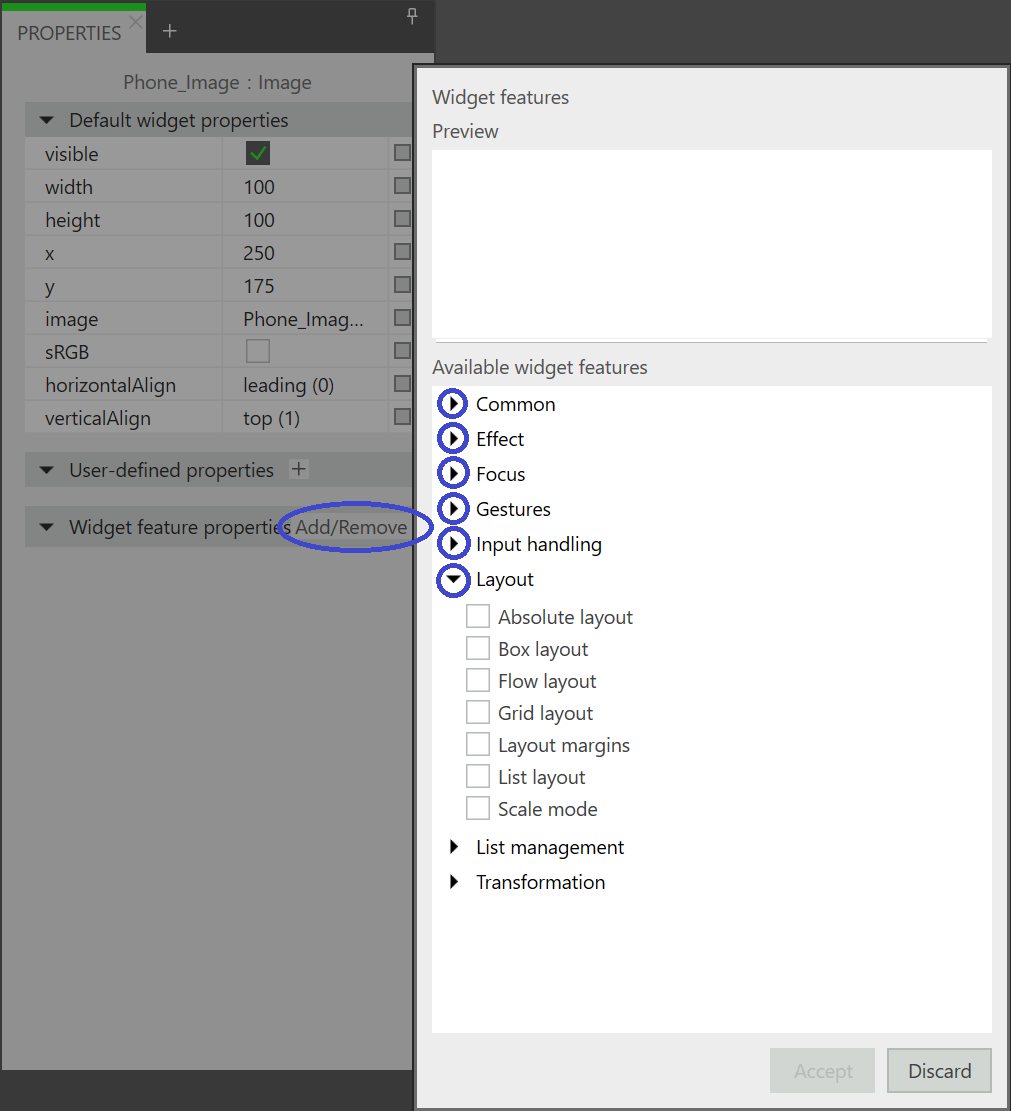
\includegraphics[scale=0.5]{figures/WidgetFeatureProperty.png}
  \captionof{figure}{Usability - Schwäche Widget Feature Properties}
  \label{fig:WidgetFeatureProperty}
\end{center}

\paragraph{Resultierende Benutzeranforderung}
Nutzer, die den Namen eines gewünschten Features wissen, müssen die Möglichkeit haben, dieses Feature aus allen Vorhandenen herauszufiltern.

\paragraph{Mehrfachselektion}
Falls bei mehreren Objekten ein Property auf den gleichen Wert gesetzt werden muss, ist es naheliegend für den Nutzer, dies durch die zeitgleiche Selektion der betroffenen Elemente zu lösen.
Aktuell bietet EB GUIDE jedoch noch keine Unterstützung für Multiselektion.
Sind zwei Elemente ausgewählt, lassen sich diese lediglich gemeinsam mit der Maus bewegen; die Properties sind, wie in \cref{fig:Mehrfachselektion} erkennbar, für den Nutzer nicht sichtbar.

\begin{center}
  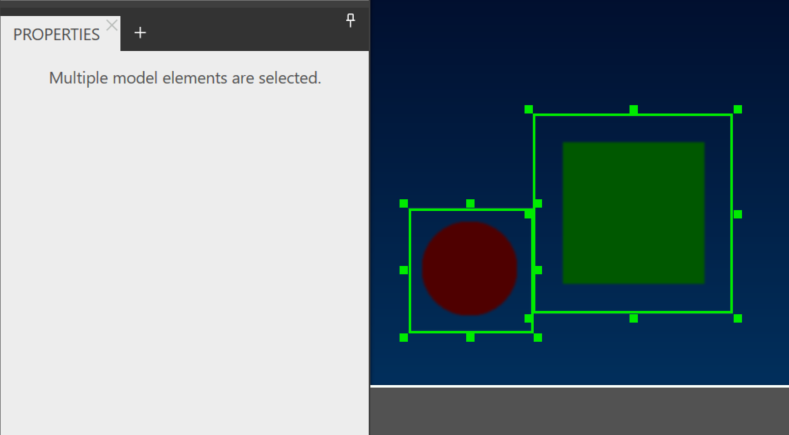
\includegraphics[scale=0.8]{figures/Mehrfachselektion.png}
  \captionof{figure}{Usability - Schwäche Mehrfachselektion}
  \label{fig:Mehrfachselektion}
\end{center}

\paragraph{Resultierende Benutzeranforderung}
Nutzer, die mehrere Objekte gleichzeitig selektiert haben, müssen die Möglichkeit haben, deren Properties nach ihren Wünschen zu ändern.

\section{Verbesserungen}
Aufgrund der zeitlichen Einschränkungen dieser Arbeit ist es nicht möglich, alle aufgeführten Schwächen weiter zu analysieren. 
Im Folgenden wird erläutert, auf welchen Grundlagen die Auswahlkriterien festgelegt werden.
Darauffolgend wird jede Verbesserung anhand dieser Kriterien eingestuft, bevor abschließend das angestrebte Design für die Verbesserungen erläutert wird.
In diesem Abschnitt wird bereits der dritte Iterationspunkt des Designprozesses angeschnitten, indem hier der Styleguide für den, im Folgenden erstellten, Prototypen, festgelegt wird. Dies geschieht auf Grundlage der bereits erläuterten Gestaltprinzipien der Usability.

\subsection{Auswahlkriterien}
Da innerhalb dieser Arbeit nur eine Iteration des Human-Centered Design Process durchgeführt werden kann, ist es wichtig, sich auf Schwächen zu fokussieren, die gewissen Kriterien gerecht werden.
Zum einen sollte bei einem Teil dieser Schwächen die Möglichkeit bestehen, innerhalb einer Iteration bereits verwertbare Ergebnisse zu erhalten.
Um jedoch auch einen längerfristigen Mehrwert für Elektrobit zu schaffen, sollte ein anderer Teil auch Verbesserungen beinhalten, die höchstwahrscheinlich weitere Iterationen zum Ausreifen benötigen.
In Anbetracht dieser Angabe und des zeitlichen Rahmens ist es also wünschenswert eine Mischung aus ein bis zwei kleineren und einer aufwändigeren Anpassung zu finden, die sich einem zusammengehörigen Test vereinbaren lassen.
Die aufwändigere soll hierbei Stoff für weitere Analysen nach Abschluss dieser Arbeit liefern, die kleineren sollen nach einer Iteration schon zu konkreteren Ergebnissen führen.

Um die Anpassungen in einem Test überprüfen zu können, ist es notwendig, sich auf zwei Prinzipien der Usability zu beschränken, die gemessen werden, da der Umfang des abschließenden Testes sonst zu umfangreich werden würde. Wie in \cref{ch:results} erläutert, ergibt sich aufgrund der Zielgruppe aktuell die Möglichkeit einer Überprüfung auf Effizienz, Wiedererkennungswert, Fehler und Zufriedenheit.
Wie bereits erwähnt, findet die Evaluierung der Zufriedenheit meist mit Fragebögen statt, die jedoch bei der Untersuchung der anderen Prinzipien nicht anwendbar sind, weshalb die objektive Zufriedenheit in dieser Arbeit nicht untersucht wird.
Die Untersuchung des Wiedererkennungswertes wäre ebenfalls möglich.
Da es sich bei der ausgewählten Gruppe jedoch um eine Mischung aus Experten und Gelegenheitsnutzern handelt, wären hier getrennte Testaufgaben für die Gelegenheitsnutzer nötig, da der Wiedererkennungswert nur bei diesem Teil der Zielgruppe untersucht werden kann.
Außerdem ist bei den im Vorherigen analysierten Schwächen keine aufgetreten, die direkt mit diesem Prinzip in Verbindung gebracht werden könnte.

Bei den durchgeführten Beobachtungen wurden jedoch Usabilityschwächen erkannt, welche sich höchstwahrscheinlich auf die Effizienz der Nutzer auswirken.
Diese Beeinträchtigung findet bei den gefunden Schwächen der Image List, der Navigation und der Widget Feature Properties dadurch statt, dass die Nutzer hier viele Menüs ausklappen oder für jedes Element - im Fall der Image List -  eine aufwändige Folge von Klicks durchlaufen müssen.
Bei der Funktion \glqq publish to template interface\grqq{} lässt sich ebenfalls vermuten, dass der nötige Rechtsklick die Nutzer in ihrer Effizienz beeinflusst.
Ebenso ist zu erwarten, dass das gleichzeitige Anpassen von Attributen durch eine funktionale Multiselektion den Modelliervorgang beschleunigt.
Ob diese Vermutungen sich wie erwartet auf das Arbeitsverhalten der Modellierer auswirken, wird mit den abschließenden Usability Tests herausgefunden.
Da für eine Messung dieses Attributes ohnehin eine Zeitmessung nötig ist, kann man währenddessen auch gut die vom System auftretenden Fehler und deren Auswirkungen auf den weiteren Arbeitsverlauf festhalten.
Die ausgewählten Verbesserungen müssen also hauptsächlich auf Effizienz und gegebenenfalls noch auf auftretende Fehler untersuchbar sein.

Zusätzlich zu den bereits genannten Kriterien, wird darauf geachtet  vor allem solche Verbesserungen zuerst zu berücksichtigen, die dem Nutzer, nach objektiven Meinungen, aktuell den größten Mehrwert liefern.

\subsection{Auswahl nach Auswahlkriterien}

\paragraph{Image List}
Die Anpassung der Befüllung der Image List ist als eine umfangreiche, aufwändige Anpassung einzuordnen.
Allerdings ist hier bereits absehbar, dass eine Anpassung die Effizienz deutlich steigern würde, da ein gruppiertes Einfügen auf jeden Fall eine Zeitersparnis mit sich bringt.
Darüber hinaus haben sich, für die Lösung dieses Problems einige Teams bereits Plug-Ins implementiert, die genau dieses Problem beheben. 
Diese sind zwar nicht Bestandteil des offiziellen Tools, werden jedoch von den internen Teams bereits routiniert benutzt, weshalb diese Anpassung auf kurze Sicht keinen Mehrwert liefern würde, sondern dies erst für neu startende Projekte der Fall wäre.
Die Anpassung der Image List würde also zum einen nicht das Kriterium erfüllen für weitere Analysen geeignet zu sein, da der Mehrwert der Anpassung bereits sehr deutlich ist.
Zum anderen existiert bereits eine temporäre Lösung für dieses Problem.

\paragraph{Navigation}
Bei der Anpassung der Navigation würde es sich um eine kleinere Anpassung handeln.
Allerdings gibt es für diese Problematik ebenfalls bereits eine Lösung, die in \cref{fig:Outline} zu sehen ist.
Es handelt sich hierbei um ein Panel in EB GUIDE Studio, welches sich Standardmäßig unterhalb des Navigationspanels befindet.
Greift man noch einmal das Beispiel aus \cref{fig:Navigation} auf, sieht die Lösung in EB GUIDE Studio für dieses Problem aktuell so aus, dass für jedes ausgewählte Objekt dessen Umgebung in der Outline angezeigt wird.
Dies funktioniert auch gut für neu eingefügte Elemente, da diese defaultmäßig nach dem Einfügen ausgewählt werden.

\begin{center}
  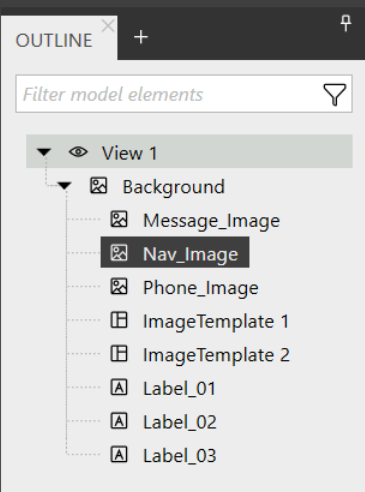
\includegraphics[scale=0.6]{figures/Outline.png}
  \captionof{figure}{Ergänzung zur Navigation in Form einer Outline}
  \label{fig:Outline}
\end{center}

Während der Beobachtung der Nutzer fällt jedoch auf, dass keiner der Nutzer diesen Outliner zu benutzen scheint, sondern lieber direkt im Widget Tree arbeitet.
An diesem Punkt wären also weitere Analysen nötig, ob manche Nutzer eventuell nichts von der Existenz dieser Funktion wissen oder ob ihnen die Nutzung zu unhandlich ist.
Aufgrund dieser ausstehenden Analysen ist diese Schwäche jedoch auch nicht für eine Überarbeitung in dieser Bachelorarbeit geeignet.

\paragraph{Template Properties}
Die Verlagerung des Hotspots für die Funktion \glqq publish to template interface\grqq{}, kann ebenfalls als eine kleine Änderung betrachtet werden.
Für diese Anpassung lässt sich mit einer Gegenüberstellung des alten und neuen Interfaces gut die benötigte Zeit der Nutzer messen, außerdem kann man hier gut herausfinden, ob die Verlagerung für die Nutzer intuitiv ist oder ob doch die alte Variante bevorzugt genutzt wird.
Es werden also bereits nach der ersten Iteration Ergebnisse auftreten, die eine konkrete Beurteilung des Vorgehens zulassen, weshalb sich diese Anpassung für den Test eignet.

\paragraph{Widget Feature Properties}
Bei dem Filter für die Widget Feature Properties handelt es sich um eine kleine bis mittelgroße Anpassung.
Der Mehrwert ist hier allerdings, vor allem für Experten, die die Namen der Features kennen, bereits absehbar.
Trotzdem eignet sich diese Anpassung ebenfalls gut für die Untersuchung der Effizienz.
Dass es eine Steigerung der Benutzerfreundlichkeit gibt, ist stark zu erwarten; ob es den Nutzern jedoch tatsächlich auch zu einem schnelleren Arbeitsablauf verhilft, ist unklar.
Zudem ist es hier interessant, ob eine komplette, neue Ergänzung im Interface von den Nutzern überhaupt selbstständig erkannt wird.
Diese Anpassung kann also als zweite kleinere Anpassung neben der Anpassung der Template Properties untersucht werden.

\paragraph{Mehrfachselektion}
Bei der Anpassung für die Mehrfachselektion besteht die Besonderheit, dass EB GUIDE hierfür, im Gegensatz zu den anderen aufgeführten Schwächen, noch keinerlei Implementierung bietet.
Es ist aktuell lediglich möglich, mehrere Elemente gleichzeitig auszuwählen und in der View zu bewegen, es existiert jedoch kein Panel, welches die aktuellen Properties anzeigt.
Dadurch ist es sehr wahrscheinlich, dass mehrere Iterationen nötig sind, um die Funktionen zufriedenstellend für den Nutzer darzustellen.
Ebenfalls ist eine Untersuchung auf Effizienz sehr gut möglich, da ein direkter Vergleich des entstehenden Zeitaufwandes mit und ohne Multiselektion getätigt werden kann.
Wegen dieser Merkmale eignet sich die Multiselektion also sehr gut als große Anpassung in dieser Arbeit.

\subsection{Design der Verbesserungen}

\paragraph{Template Properties}

Wie in \cref{fig:TemplateProperties_Adaption} zu sehen, ist für diese Änderung keine tatsächliche Abwandlung des Designs notwendig, da sich lediglich der Hotspot verlagert.
Trotzdem werden hier einige Gestaltprinzipien der Usability berücksichtigt.
Die nötige Rückmeldung an den Nutzer geschieht durch die Änderung der Farbe des Kreises.
Dieses Verhalten ist bereits vorhanden, allerdings wird durch die bisherige Lösung eine minimale Verletzung des Mappings verursacht, da durch eine Interaktion mit dem Quadrat eine Rückmeldung mithilfe des Kreises erzeugt wurde. 
Das Mapping wird also durch das hier vorgestellte Design verbessert.

Im Gegensatz dazu wird jedoch durch die Anpassung die interne Konsistenz verletzt, da die Interaktion mit den Template Properties auch noch an anderen Stellen möglich ist, wo die Anpassung zum aktuellen Zeitpunkt noch nicht integriert werden kann.
Diese Verletzung kann jedoch nach Validierung durch den Usability Test im Nachhinein angepasst werden oder der Hotspot auf dem Kreis könnte als zusätzliche Ergänzung für Expertennutzer existieren.

\begin{center}
  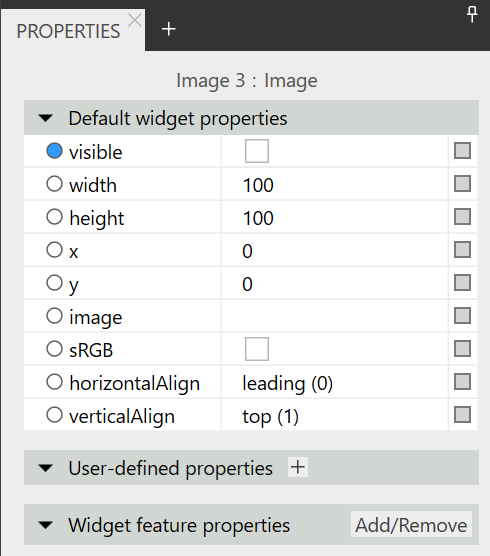
\includegraphics[scale=0.8]{figures/TemplateProperties_Adaption.png}
  \captionof{figure}{Verbesserung Template Properties}
  \label{fig:TemplateProperties_Adaption}
\end{center}

\newpage
\paragraph{Widget Feature Properties}
Für das Hinzufügen einer Filterfunktion ist das Einfügen einer Filterleiste in das Interface, wie in \cref{fig:FeatureProperty_Adaption} zu sehen, nötig.
Teil a) der Abbildung zeigt hier zur Erinnerung noch einmal die bestehende Implementierung, in Teil b) ist der ergänzte Filter zu sehen, der in c) live nach dem eingegebenen Begriff filtert.

\begin{figure}[H]
  \centering
  \subfloat[][]{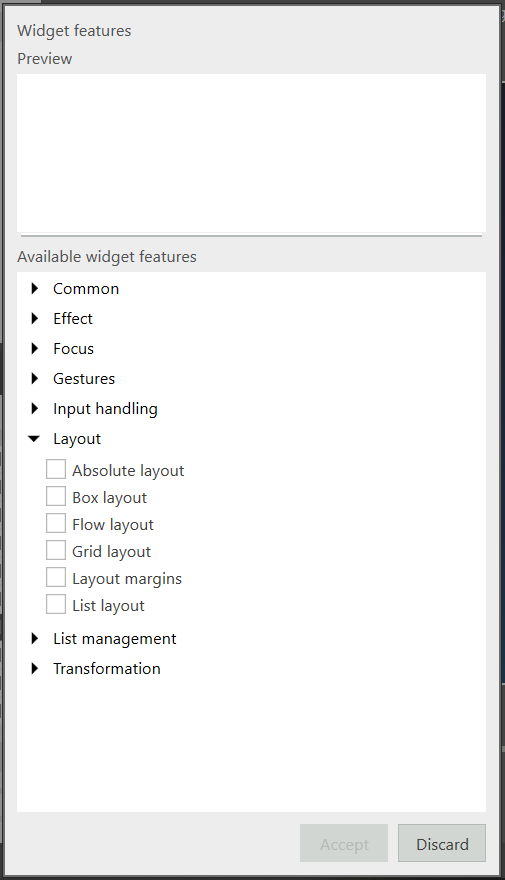
\includegraphics[width=0.28\linewidth]{figures/WidgetFeatureProperty_Before.PNG}}%
  \qquad
  \subfloat[][]{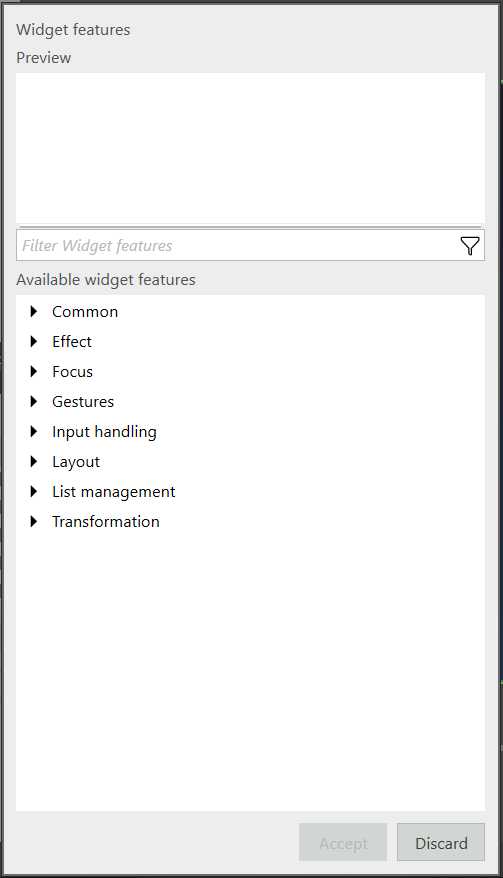
\includegraphics[width=0.28\linewidth]{figures/WidgetFeatureProperty_Adaption.PNG}}%
 \qquad
  \subfloat[][]{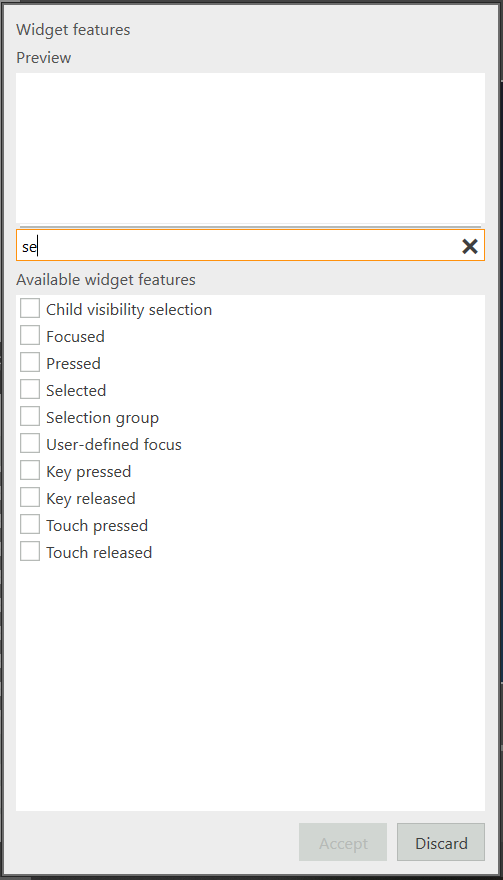
\includegraphics[width=0.28\linewidth]{figures/WidgetFeatureProperty_Live.PNG}}%
  \captionof{figure}{Verbesserung Feature Property Properties}
  \label{fig:FeatureProperty_Adaption}
\end{figure}

Als Gestaltprinzip der Usability wird hier, zum einen die ästehtische, funktionale und interne Konsistenz des Designs, zum anderen Such- und Filterfunktionen, die in der Benutzeroberfläche von EB GUIDE Verwendung finden, gewahrt.
Dadurch ergibt sich automatisch eine externe Konsistenz, da das bereits bestehende Design dieser Leisten von Elektrobit an das Design bereits bekannter Suchleisten angelehnt wurde.

Aktuell wird die in \cref{ch:gestalt} erwähnte Problematik der Sichtbarkeit in komplexen Systemen durch die ausklappbaren Menüs gelöst.
Dies führt jedoch in diesem konkreten Fall häufig dazu, dass all diese Menüs, während der Suche nach dem richtigen Feature, aufgeklappt werden müssen.
Der geplante Filter soll die Nutzer insofern unterstützen, dass sie die Sichtbarkeit der Features nach ihren eigenen Bedingungen anpassen können, wenn sie wissen, nach welchem Feature sie suchen.

Das Gestaltprinzip der Affordanz wird durch den ausgegrauten Text in der Filterleiste berücksichtigt, da der Nutzer durch den Text \glqq Filter Widget features\grqq{} die direkte Aufforderung erhält, was hier getan werden kann.
Zum anderen bekommt er durch den grauen Text suggeriert, dass hier etwas anklickbar ist und eine Eingabe getätigt werden kann.

Die Rückmeldung, die für den Nutzer sehr wichtig ist, erfolgt durch die Tatsache, dass der Filter live auf die Änderungen des Nutzers reagiert, es also eine sehr schnelle Anpassung der Liste der Features gibt.

\paragraph{Mehrfachselektion}
Um die Anpassung der Properties bei Mehrfachselektion zu ermöglichen, ist es nötig, ein Property Panel anzuzeigen, wie in \cref{fig:Mehrfachselektion_Adaption} zu sehen.
Wie bei der normalen Auswahl eines Elementes werden dort Properties wie width/height und die Koordinaten angezeigt, zusätzlich ist es mit den neuen Alignment Actions noch möglich, die ausgewählten Elemente aneinander auszurichten.
Diese Funktion gibt es bisher in EB GUIDE Studio noch nicht, erschien jedoch im Kontext der Mehrfachselektion eine geeignete Ergänzung zu sein.

\begin{center}
  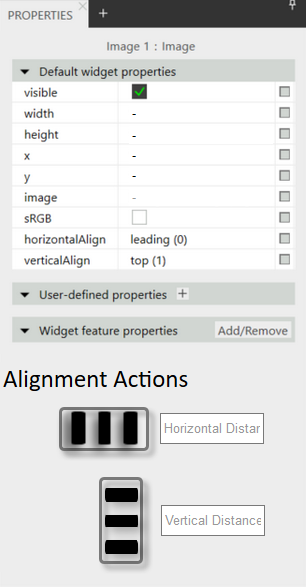
\includegraphics[scale=0.8]{figures/Mehrfachselektion_Adaption02.png}
  \captionof{figure}{Verbesserung Mehrfachselektion}
  \label{fig:Mehrfachselektion_Adaption}
\end{center}

Auch hier wird die ästhetische, funktionale und interne Konsistenz bei den Textfeldern der Properties gewahrt, da sie exakt so aussehen, wie die bereits Bekannten bei der Auswahl eines Elements.
Externe Konsistenz wird durch die Striche gewahrt, die als Platzhalter bei den Values der Properties fungieren, wenn die ausgewählten Elemente zum Beispiel bei der x-Koordinate unterschiedliche Werte aufweisen.
In EB GUIDE ist es allgemein so, dass nur die Properties sichtbar sind, die für die aktuell ausgewählten Elemente relevant und veränderbar sind.
Diese Einschränkung der Sichtbarkeit ist dementsprechend auch bei der Multiselektion zu beachten.
Wenn also beispielsweise ein Bild und ein Text gleichzeitig ausgewählt sind, ist es nicht nötig, eine Text Property bereitzustellen, da diese nicht bei beiden Elementen anpassbar wäre.

Das Prinzip der Affordanz wird bei den Buttons für die Alignment Actions berücksichtigt, indem diese einen Schatten bekommen, um sie klickbar erscheinen zu lassen.
Ebenfalls wird es wieder bei den Textfeldern neben den Buttons berücksichtigt, wie es auch bei der Filterfunktion bereits der Fall ist.

Eine Rückmeldung an den Nutzer, dass seine Eingaben erfolgreich waren, erfolgt durch die sofortige Veränderung der Elemente im View, entweder durch Änderungen der Position, oder der Breite und Höhe.

Zusätzlich dazu soll es noch möglich sein, Bilder in Templates über Multiselektion einzufügen.
Das Design hierfür ist in \cref{fig:Mehrfachselektion_Adaption_Template} zu sehen.
Die Design Prinzipien werden hier auf die gleiche Art und Weise berücksichtigt, wie es bei den Buttons für die Alignment Actions bereits erläutert wurde.
In diesem Fall ist jedoch kein Textfeld nötig, da hier kein Abstand oder ähnliches Angegeben werdenmuss.
Bei einem Klick auf den Button wird ein ausgewältes Bild in ein gleichzeitig ausgewähltes Template eingefügt.

\begin{center}
  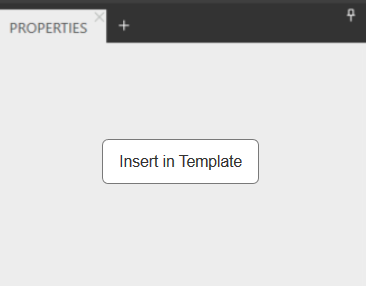
\includegraphics[scale=0.8]{figures/Mehrfachselektion_Adaption03.png}
  \captionof{figure}{Verbesserung Mehrfachselektion Einfügen in Template}
  \label{fig:Mehrfachselektion_Adaption_Template}
\end{center}



